\documentclass[11pt,a4paper,onecolumn]{article}
\usepackage[T1]{fontenc}
\usepackage[utf8]{inputenc}
\usepackage{lmodern,microtype}
\usepackage[margin=1in]{geometry}
\usepackage{amsmath,amssymb,amsthm,mathtools}
\usepackage{booktabs,tabularx,array,enumitem,float,needspace}
\usepackage[section]{placeins}
\usepackage{tikz}
\usetikzlibrary{arrows.meta,positioning,fit,calc}
\usepackage[framemethod=default]{mdframed}
\usepackage{xcolor}
\usepackage[hidelinks]{hyperref}
\usepackage[nameinlink,noabbrev]{cleveref}
\usepackage{fancyhdr}
\hypersetup{pdftitle={An Authenticated Live Sequencer Stream},
pdfsubject={Regional PoS SMR with Sync HotStuff; cross-region CFT remains unfinished}}
\setlength{\headheight}{14pt}
\pagestyle{fancy}\fancyhf{}
\lhead{\small An authenticated live sequencer stream}\rhead{\small Version 2 / working draft}
\cfoot{\thepage}
\setlength{\emergencystretch}{2em}
\setlist{nosep,leftmargin=*}
\newcolumntype{Y}{>{\raggedright\arraybackslash}X}
\newcommand{\Hash}{\mathsf H}
\newcommand{\Sig}{\mathsf{Sign}}
\newcommand{\QC}{\mathsf{QC}}
\newcommand{\gv}{v_{\mathrm G}}
\newcommand{\lv}{v_{\mathrm L}}
\newcommand{\pre}{\preceq}
\newcommand{\wt}{\operatorname{wt}}
\newcommand{\rank}{\operatorname{rank}}
\newcommand{\Tag}[1]{\ensuremath{\mathsf{#1}}}
\newcommand{\Proc}[1]{\textnormal{\textsc{#1}}}
\newtheorem{definition}{Definition}[section]
\newtheorem{assumption}[definition]{Assumption}
\newtheorem{lemma}[definition]{Lemma}
\newtheorem{theorem}[definition]{Theorem}
\newcounter{protocol}
\newenvironment{protocol}[2]{\refstepcounter{protocol}\label{#1}
\begin{mdframed}[nobreak=true,linewidth=.6pt,skipabove=9pt,skipbelow=9pt,
innertopmargin=7pt,innerbottommargin=7pt]\small
\noindent\textbf{Protocol \theprotocol. #2}\par\smallskip}{\end{mdframed}}
\crefname{protocol}{Protocol}{Protocols}
\Crefname{protocol}{Protocol}{Protocols}
\crefname{definition}{Definition}{Definitions}
\crefname{assumption}{Assumption}{Assumptions}
\crefname{lemma}{Lemma}{Lemmas}
\crefname{theorem}{Theorem}{Theorems}
\title{An Authenticated Live Sequencer Stream\\
\large Regional PoS SMR with Sync HotStuff}
\author{}\date{28 September 2026}
\begin{document}
\maketitle
\begin{abstract}
We organize a live sequencing service into regional state machine replication
(SMR) and a future cross-region crash-fault-tolerant (CFT) layer. A stable
interface exposes authenticated mini-blocks and confirmed prefixes without
exposing the underlying BFT messages. We instantiate the regional layer using
L1 stake weights, an installed producer list, and the chained synchronous
Sync HotStuff protocol. Certification permits continuous proposal pipelining;
commitment and leader replacement follow separate timing rules. Leader push
and peer poll-fetch deliver the resulting stream to proposer $P$. We give
the regional algorithms, safety and progress arguments, and their communication
and latency costs. Cross-region election, rotation and global commitment remain
unfinished.
\end{abstract}

\section{Two-Layer Structure}\label{sec:architecture}
Each region runs an SMR instance whose log contains batches of mini-blocks.
The regional replicas agree on their contents and order. Proposer $P$ verifies
the resulting stream, executes transactions, and performs downstream
publication. Sequencers may execute privately to choose an order, but this
service certifies ordering rather than EVM execution.

The intended outer protocol treats a regional SMR as one logical participant:
its state transitions are replicated and its accepted outputs are authenticated
by the region. It will select the active production region and preserve one
stream across regional failures. This abstraction is conditional on the
regional safety assumptions; a violation of inner synchrony is not
automatically a crash-only outer failure.

\begin{figure}[H]\centering
% Application-level layout retained from figures/v2/architecture.tex.
% Solid arrows carry data or configuration; dashed arrows are pull requests.
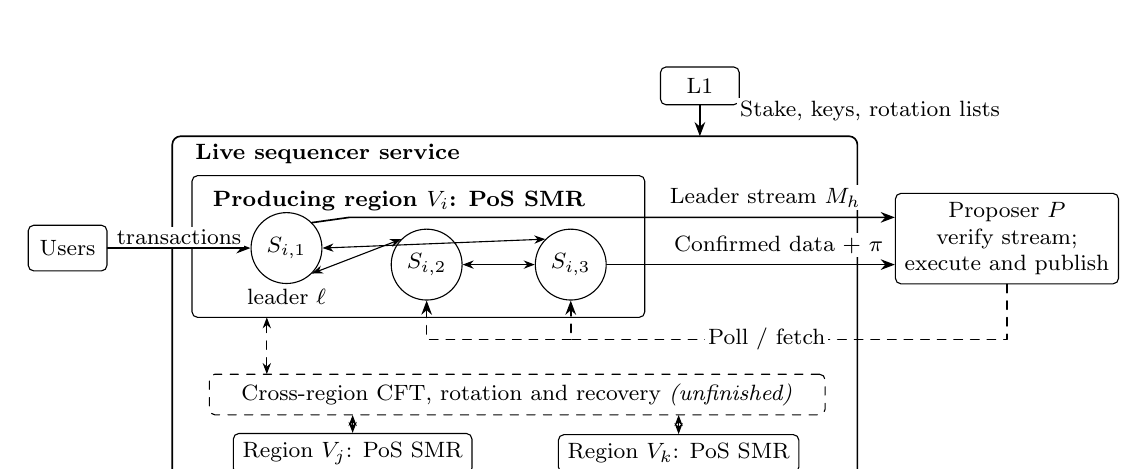
\begin{tikzpicture}[
  x=1cm,y=1cm,font=\footnotesize,line cap=round,line join=round,
  box/.style={draw,rounded corners=2pt,align=center,fill=white},
  seq/.style={draw,circle,minimum size=9mm,inner sep=1pt,fill=white},
  flow/.style={-{Stealth[length=1.8mm]},semithick},
  pull/.style={flow,dashed},
  control/.style={{Stealth[length=1.4mm]}-{Stealth[length=1.4mm]},thin},
  lab/.style={fill=white,inner sep=1pt,align=center}
]
  \draw[rounded corners=3pt,semithick] (1.85,0) rectangle (10.55,4.35);
  \node[anchor=west,font=\footnotesize\bfseries] at (2.02,4.12)
    {Live sequencer service};
  \draw[rounded corners=2pt] (2.10,2.05) rectangle (7.85,3.85);
  \node[anchor=north west,font=\footnotesize\bfseries] at (2.24,3.78)
    {Producing region $V_i$: PoS SMR};
  \node[box,minimum width=1.0cm,minimum height=.58cm] (users) at (.52,2.93) {Users};
  \node[seq] (leader) at (3.30,2.93) {$S_{i,1}$};
  \node[lab,anchor=north] at (3.30,2.45) {leader $\ell$};
  \node[seq] (peerone) at (5.08,2.72) {$S_{i,2}$};
  \node[seq] (peertwo) at (6.91,2.72) {$S_{i,3}$};
  \draw[control] (leader.south east) -- (peerone.north west);
  \draw[control] (leader.east) -- (peertwo.north west);
  \draw[control] (peerone.east) -- (peertwo.west);
  \draw[flow] (users.east) -- node[lab,above] {transactions} (leader.west);

  \node[box,minimum width=1.8cm,minimum height=1.08cm] (proposer) at (12.45,3.05)
    {Proposer $P$\\verify stream;\\execute and publish};
  \draw[flow] (leader.north east) -- (4.10,3.32) -- ($(proposer.west)+(0,.27)$);
  \node[lab] at (9.38,3.57) {Leader stream $M_h$};
  \draw[flow] (peertwo.east) -- ($(proposer.west)+(0,-.33)$);
  \node[lab] at (9.55,2.97) {Confirmed data + $\pi$};
  \draw[pull] (proposer.south) -- (12.45,1.77) -- (6.91,1.77) -- (peertwo.south);
  \draw[pull] (6.91,1.77) -- (5.08,1.77) -- (peerone.south);
  \node[lab] at (9.40,1.77) {Poll / fetch};

  \node[box,dashed,minimum width=7.82cm,minimum height=.51cm] (outer) at (6.23,1.07)
    {Cross-region CFT, rotation and recovery \emph{(unfinished)}};
  \draw[control,dashed] (3.05,2.05) -- (3.05,1.33);
  \node[box,minimum width=2.95cm,minimum height=.43cm] (rj) at (4.14,.32)
    {Region $V_j$: PoS SMR};
  \node[box,minimum width=2.95cm,minimum height=.43cm] (rk) at (8.28,.32)
    {Region $V_k$: PoS SMR};
  \draw[control,dashed] (4.14,.81) -- (rj.north);
  \draw[control,dashed] (8.28,.81) -- (rk.north);

  \node[box,minimum width=1.0cm,minimum height=.48cm] (lone) at (8.55,4.99) {L1};
  \draw[flow] (lone.south) -- (8.55,4.35);
  \node[lab,anchor=west] at (9.02,4.67) {Stake, keys, rotation lists};
\end{tikzpicture}

\caption{The application and its two layers. Solid paths implement regional
production and delivery; dotted components mark unfinished cross-region work.
Sequencer icons illustrate roles, not a committee-size assumption.}
\label{fig:architecture}
\end{figure}

\textbf{Open outer layer.}
Cross-region CFT election, replicated-state transitions, authority transfer,
regional crash/recovery and global finality are not specified here.
A regional confirmed prefix is immutable within its authorized session.
Making it irrevocable across region changes requires the outer protocol to
inherit that prefix. No local certificate by itself settles this outer rule.

\section{Model and Service Definitions}\label{sec:model}
\subsection{Configuration, network and adversary}
L1 supplies a finalized stake configuration: regional membership, public keys,
weights, producer lists and protocol parameters. Region $V_i$ contains
sequencers $S_{i,j}$ of weights $\omega_{i,j}=w_{S_{i,j}}>0$; its total stake
is $W_i$. Write $\wt(U)$ for the sum of weights in $U$. Its cyclic list
$\mathcal L_i$ determines the leader of local view $v$:
\[
 \ell_i(v)=\mathcal L_i[v\bmod |V_i|].
\]
Votes are stake-weighted; this once-per-identity list does not imply
stake-proportional producer frequency. A regional session starts from a
commonly authenticated configuration and initial stream checkpoint.
All statements bind this session. Membership and weights remain fixed
during the session.

\begin{assumption}[Regional execution]\label[assumption]{ass:network}
Faulty stake in every analyzed region is below $W_i/3$. Correct members retain
their protocol state and participate throughout the execution. Their
authenticated messages, with the data and verification needed to process
them, arrive within $\Delta_R$. Actual good-case delay is
$\delta_R\leq\Delta_R$. Local clocks measure durations at the same rate;
steady-state rounds do not require a common wall clock. Signatures cannot
be forged and hash commitments cannot be opened inconsistently.
\end{assumption}

Faults may include permanent omission; recovering replicas restore their
state before participating. Arbitrary mobile outages or violations of the
regional delay bound are outside this instantiation. Capacity and batch
limits must make the complete-message bound feasible. A live consumer has
an eventually usable path to retained honest data holders. For bounded
latency analysis its one-way complete-message bound is $\Delta_P$, with
actual delay $\delta_P$.

\subsection{An authenticated live mini-block stream}\label{sec:stream}
A mini-block at height $h$ has the content and authentication structure
\[
 M_h=(H_h,\mathcal X_h,\Sig_\ell(\Tag{ORDER},H_h)),
 \qquad q_h=\Hash(\Tag{MINIBLOCK},H_h).
\]
Here $\mathcal X_h$ is the ordered list of raw transaction bytes. Header $H_h$
binds height $h$, predecessor $q_{h-1}$, a commitment to $\mathcal X_h$, and
the producer's authorization context. The initial predecessor is supplied by
the authenticated checkpoint. Local view and attempt metadata, when needed,
belong to that authorization context; consumers do not use them as the
service's control interface. The order, multiplicities and lengths of the
transaction lists are committed. No execution or receipt root is required.
Mini-block identity is determined by its header and transaction bytes;
alternative valid signature or receipt encodings are evidence for the same
object, not different stream entries.

The public confirmation interface is
\[
 \Tag{Deliver}(P,h,M_h,\pi_h),\qquad
 \Proc{VerifyStream}(M_h,\pi_h;\Gamma)\in\{0,1\},
\]
where $\Gamma$ is the verified configuration and preceding stream context.
The receipt $\pi_h$ authenticates membership of $M_h$ in a confirmed prefix.
Its encoding is implementation-dependent: replacing the BFT engine changes
the receipt verifier, not the meaning of \Tag{Deliver}. Raw data may arrive
earlier and is buffered until the receipt and predecessor are verified.

\begin{definition}[Regional live stream]\label{def:stream}
Within an authorized regional session, the service provides:
\begin{enumerate}[label=(\roman*)]
\item \emph{Authenticity and integrity.} Every delivered mini-block has valid
producer authorization and matches its committed contents and predecessor.
\item \emph{Safety.} Correct receivers' delivered logs are prefix comparable,
and a receiver's delivered log never shrinks.
\item \emph{Liveness.} Under the regional execution and service assumptions,
the confirmed stream grows, and every confirmed mini-block is eventually
delivered to each live subscribed receiver.
\end{enumerate}
\end{definition}
This definition refers to regional confirmation. The outer layer must provide
the corresponding cross-region prefix guarantee. Transaction selection and
execution validity are separate from stream integrity.

\subsection{State machine replication and its application}\label{sec:smr}
\begin{definition}[SMR]\label{def:smr}
A deterministic state machine processes a sequence of submitted commands.
An SMR protocol implements a committed command log satisfying:
\begin{itemize}
\item \emph{Safety:} no two correct replicas commit different values at the
same log position; committed prefixes are never withdrawn.
\item \emph{Liveness:} every well-formed request submitted by a correct client
is eventually committed by all correct replicas, under the stipulated
execution conditions.
\end{itemize}
Correct replicas apply commands in log order and hence produce the same state
and output after the same prefix.
\end{definition}
These are the consensus-community SMR properties used by Sync
HotStuff~\cite{synchotstuff}; deterministic execution follows the standard
state-machine approach~\cite{schneider}.

For this application a command is an ordered batch of mini-block
\emph{contents}, before protocol positions and views are assigned. A consensus
proposal places that command on a particular parent and authenticates the
resulting mini-blocks. Thus a command differs from a view-specific candidate:
a replaced candidate is not a promise that every competing proposal will
commit. The committed block chain determines both the command-log projection
and the mini-block-stream projection. Transaction selection belongs to the
producer; this service orders the submitted batch contents. A correct-client
submission keeps its pending command available until confirmation.

\begin{assumption}[Input service and retention]\label[assumption]{ass:service}
Batch construction and offered load fit the configured service capacity;
honest leaders continuously obtain valid batches, using an empty-transaction
mini-block when idle. For request-level SMR liveness, each persistently
submitted eligible batch reaches a sufficiently long honest-serving interval,
and the input selection in that interval does not starve it.
Committed contents and receipts remain available at honest regional members.
\end{assumption}
The input-service premise concerns batches submitted to the SMR, not every
transaction waiting in a producer's mempool. The consensus protocol itself
guarantees stream progress; inclusion of a particular request additionally
uses this premise. A Byzantine producer that keeps producing valid batches
is not removed solely because it omits a particular transaction.

\section{Regional PoS SMR: Sync HotStuff and Chaining}\label{sec:protocol}
\subsection{L1-backed participation and weighted certificates}
Permissionless admission is delegated to L1's staking rules. The regional
engine runs on one activated snapshot of that stake table, rather than on a
privately appointed list. A new stake snapshot requires a preserved checkpoint
and safe activation; that transition is left with the unfinished inter-session
control layer. Slashing evidence does not change the current denominator
mid-execution. This is a PoS regional engine, not a completed dynamic
permissionless reconfiguration protocol.

The generic permissioned-to-PoS compiler of Komatovic et al.~\cite{poscompiler}
provides the broader epoch-and-certification framework. Its preservation
theorem assumes a base protocol with the corresponding properties under
partial synchrony, so it does not directly prove the synchronous construction
below. We establish the weighted fixed-snapshot case.

From here fix one region. A batch block $B_k$ occupies log position $k$,
points to its parent $B_{k-1}$, and carries a bounded, nonempty consecutive
range of mini-blocks. An idle mini-block may contain zero transactions.
Its digest binds the parent and ordered mini-block identifiers;
signature encodings are witnesses, not distinct values. The root $B_0$ is
the initial checkpoint. Two blocks conflict if neither extends the other.

A certificate $Q_v(B_k)$ consists of votes on $B_k$ in view $v$ by distinct
members of total weight $>2W_i/3$. Rank certificates lexicographically by
$(v,k)$, with the root initially below every ordinary certificate. A block
can be re-certified in a later view without changing its mini-blocks or
original producer signatures. Certificate view and original authorship view
therefore need not coincide.

This vote threshold is the conservative weighted adaptation of Sync HotStuff's
majority certificate: every vote certificate contains an honest signer, and honest
stake alone can form one. Its temporal argument below supplies safety;
we do not transfer a count-based fault bound to stake without this check.
Producer and vote signatures bind the session, view, position and block
digest. An honest member votes at most once per view and position.
Previously verified parent data can be cached, but a member validates the
complete missing chain and batch before voting.

\subsection{Normal operation and the chained pipeline}
We instantiate the standard-synchronous protocol in Section II, Figures 1--2,
of the \emph{4 May 2020 revision} of Sync HotStuff~\cite{synchotstuff}.
The native \Tag{NEWVIEW} step below is important: it re-certifies the inherited
anchor before fresh proposals. Views change on protocol events; a healthy
leader continues proposing while commitment timers overlap.

\begin{protocol}{alg:steady}{Steady-state regional SMR}
\textbf{In view $v$, with leader $\ell_i(v)$ and a current-view certified anchor:}
\begin{enumerate}[label=\textbf{S\arabic*.}]
\item \textbf{Propose.} On obtaining $Q_v(B_{k-1})$, the leader forms the
next valid batch, signs its mini-blocks and proposal, and sends
$(B_k,Q_v(B_{k-1}))$ to the region. The batch extends that exact parent.
\item \textbf{Echo and vote.} On the first valid proposal at $(v,k)$, received
directly or relayed, check producer authority, the current-view parent
certificate, contents and prefix links. If still in view $v$ and no leader
equivocation is known, forward the signed proposal, multicast a vote, and
start a $2\Delta_R$ timer for this block.
\item \textbf{Pipeline.} Matching votes form $Q_v(B_k)$. The leader may
immediately propose its child. Neither a running commit timer nor $P$'s
acknowledgement blocks this step.
\item \textbf{Commit.} If the timer expires while still in view $v$ without
equivocation, commit the block and all uncommitted ancestors in order.
Retain their contents and emit the confirmation of \cref{sec:receipt}.
The certificate is available by this time under \cref{ass:network};
otherwise no confirmation is emitted.
\end{enumerate}
\end{protocol}

All forwarding retains the original signatures. A parent certificate from an
older view cannot bypass the current-view requirement. Proposal validity
includes increasing batch and mini-block positions, correct prefix commitments,
and the configured batch-size limit. Nodes process received conflict/quit
evidence before a timer expiring at the same instant.

\begin{figure}[H]\centering
% Positions show causal order, not a scale proportional to network delay.
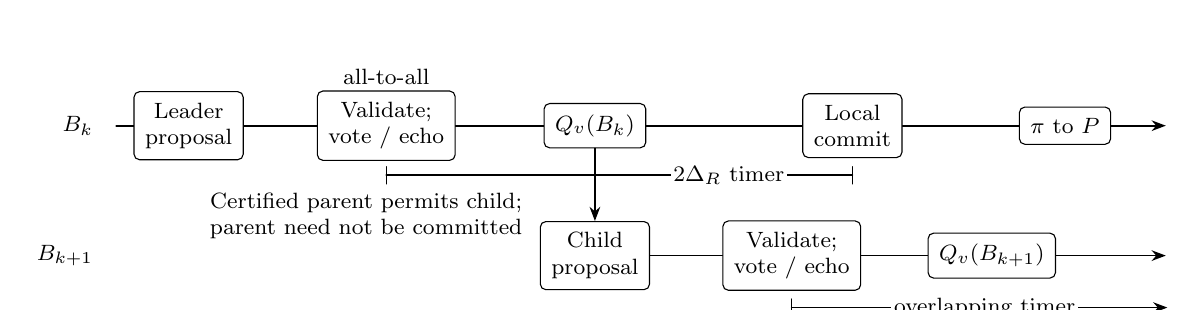
\begin{tikzpicture}[
  x=1cm,y=1cm,font=\footnotesize,line cap=round,line join=round,
  flow/.style={-{Stealth[length=1.8mm]},semithick},
  event/.style={draw,rounded corners=2pt,align=center,fill=white,inner sep=4pt},
  lab/.style={fill=white,inner sep=1pt,align=center}
]
  \node[anchor=east] at (.48,2.55) {$B_k$};
  \draw[flow] (.65,2.55) -- (13.98,2.55);
  \node[event] (prop) at (1.57,2.55) {Leader\\proposal};
  \node[event] (vote) at (4.08,2.55) {Validate;\\vote / echo};
  \node[event] (qc) at (6.73,2.55) {$Q_v(B_k)$};
  \node[event] (commit) at (10.00,2.55) {Local\\commit};
  \node[event] (receipt) at (12.70,2.55) {$\pi$ to $P$};
  \node[lab] at (4.08,3.17) {all-to-all};
  \draw[semithick] (4.08,1.92) -- (10.00,1.92);
  \draw (4.08,1.81) -- (4.08,2.03);
  \draw (10.00,1.81) -- (10.00,2.03);
  \node[lab] at (8.43,1.92) {$2\Delta_R$ timer};

  \node[anchor=east] at (.48,.90) {$B_{k+1}$};
  \draw[flow] (6.73,.90) -- (13.98,.90);
  \node[event] (child) at (6.73,.90) {Child\\proposal};
  \node[event] (cvote) at (9.23,.90) {Validate;\\vote / echo};
  \node[event] (cqc) at (11.77,.90) {$Q_v(B_{k+1})$};
  \draw[flow] (qc.south) -- (child.north);
  \node[lab,anchor=east] at (5.85,1.40) {Certified parent permits child;\\parent need not be committed};
  \draw[semithick] (9.23,.24) -- (13.65,.24);
  \draw (9.23,.13) -- (9.23,.35);
  \draw[flow] (13.65,.24) -- (14.00,.24);
  \node[lab] at (11.68,.24) {overlapping timer};
\end{tikzpicture}

\caption{Certification advances the proposal chain while commitment timers
overlap. A vote certificate and a confirmed-stream receipt have different meanings.}
\label{fig:pipeline}
\end{figure}

\Cref{fig:pipeline-communication} expands this pipeline into the message flow
among four regional sequencers. The drawing does not assign them equal stake.
Vote certificates require weight $>2W_i/3$; post-commit receipts require
matching endorsements of weight $>W_i/3$.

\begin{figure}[H]\centering
% Four-member steady-state message sequence.  Time runs from top to bottom;
% vertical distances show causal order rather than measured network delay.
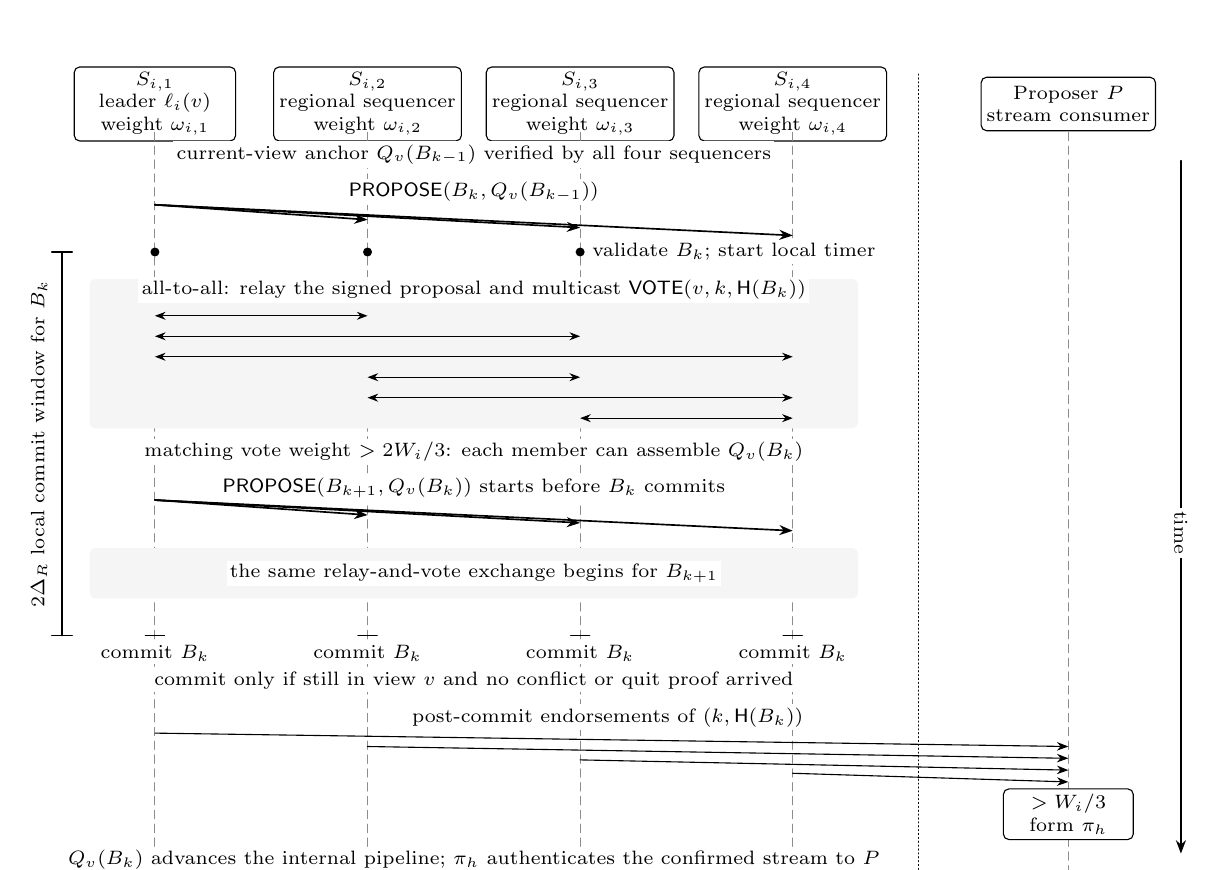
\begin{tikzpicture}[
  x=1cm,y=1cm,font=\scriptsize,line cap=round,line join=round,
  party/.style={draw,rounded corners=2pt,align=center,fill=white,
    minimum width=2.05cm,minimum height=.68cm,inner sep=2pt},
  lifeline/.style={densely dashed,thin,black!45},
  proposal/.style={-{Stealth[length=1.7mm]},semithick},
  exchange/.style={{Stealth[length=1.35mm]}-{Stealth[length=1.35mm]},thin},
  confirm/.style={-{Stealth[length=1.45mm]},thin},
  milestone/.style={circle,fill=black,inner sep=1.15pt},
  lab/.style={fill=white,inner sep=1.2pt,align=center}
]
  \def\xa{1.55}
  \def\xb{4.25}
  \def\xc{6.95}
  \def\xd{9.65}
  \def\xp{13.15}

  % Participants and lifelines.
  \node[party] at (\xa,10.30) {$S_{i,1}$\\leader $\ell_i(v)$\\weight $\omega_{i,1}$};
  \node[party] at (\xb,10.30) {$S_{i,2}$\\regional sequencer\\weight $\omega_{i,2}$};
  \node[party] at (\xc,10.30) {$S_{i,3}$\\regional sequencer\\weight $\omega_{i,3}$};
  \node[party] at (\xd,10.30) {$S_{i,4}$\\regional sequencer\\weight $\omega_{i,4}$};
  \node[party,minimum width=1.65cm] at (\xp,10.30)
    {Proposer $P$\\stream consumer};
  \foreach \x in {\xa,\xb,\xc,\xd,\xp}
    \draw[lifeline] (\x,9.94) -- (\x,.52);
  \draw[densely dotted] (11.25,10.68) -- (11.25,.45);
  \draw[proposal] (14.58,9.58) -- node[lab,right,rotate=-90] {time} (14.58,.78);

  % The current-view anchor is already common before the next proposal.
  \node[lab] at (5.60,9.66)
    {current-view anchor $Q_v(B_{k-1})$ verified by all four sequencers};

  % B_k proposal fan-out.
  \node[lab] at (5.60,9.18)
    {$\Tag{PROPOSE}(B_k,Q_v(B_{k-1}))$};
  \draw[proposal] (\xa,9.02) -- (\xb,8.83);
  \draw[proposal] (\xa,9.02) -- (\xc,8.73);
  \draw[proposal] (\xa,9.02) -- (\xd,8.63);
  \foreach \x in {\xa,\xb,\xc,\xd}
    \node[milestone] at (\x,8.42) {};
  \node[lab,anchor=east] at (10.75,8.42)
    {validate $B_k$; start local timer};

  % Explicit all-to-all exchange for B_k.  A bidirectional edge represents
  % the proposal relays and vote multicasts between that pair of members.
  \path[fill=black!4,rounded corners=2pt] (.72,6.18) rectangle (10.48,8.08);
  \node[lab] at (5.60,7.94)
    {all-to-all: relay the signed proposal and multicast $\Tag{VOTE}(v,k,\Hash(B_k))$};
  \draw[exchange] (\xa,7.61) -- (\xb,7.61);
  \draw[exchange] (\xa,7.35) -- (\xc,7.35);
  \draw[exchange] (\xa,7.09) -- (\xd,7.09);
  \draw[exchange] (\xb,6.83) -- (\xc,6.83);
  \draw[exchange] (\xb,6.57) -- (\xd,6.57);
  \draw[exchange] (\xc,6.31) -- (\xd,6.31);

  % Every member sees the multicast votes; certification immediately opens
  % the next pipeline position even though B_k's timers are still running.
  \foreach \x in {\xa,\xb,\xc,\xd}
    \node[milestone] at (\x,5.88) {};
  \node[lab] at (5.60,5.88)
    {matching vote weight $>2W_i/3$: each member can assemble $Q_v(B_k)$};

  \node[lab] at (5.60,5.43)
    {$\Tag{PROPOSE}(B_{k+1},Q_v(B_k))$ starts before $B_k$ commits};
  \draw[proposal] (\xa,5.27) -- (\xb,5.08);
  \draw[proposal] (\xa,5.27) -- (\xc,4.98);
  \draw[proposal] (\xa,5.27) -- (\xd,4.88);

  \path[fill=black!4,rounded corners=2pt] (.72,4.02) rectangle (10.48,4.66);
  \node[lab] at (5.60,4.34)
    {the same relay-and-vote exchange begins for $B_{k+1}$};

  % The B_k commit window overlaps communication for B_{k+1}.
  \draw[semithick] (.37,8.42) -- (.37,3.55);
  \draw[semithick] (.24,8.42) -- (.50,8.42);
  \draw[semithick] (.24,3.55) -- (.50,3.55);
  \node[lab,rotate=90] at (.08,5.98) {$2\Delta_R$ local commit window for $B_k$};
  \foreach \x in {\xa,\xb,\xc,\xd} {
    \draw[semithick] ($(\x,3.55)+(-.12,0)$) -- ($(\x,3.55)+(.12,0)$);
    \node[lab,anchor=north] at (\x,3.48) {commit $B_k$};
  }
  \node[lab] at (5.60,2.98)
    {commit only if still in view $v$ and no conflict or quit proof arrived};

  % Post-commit endorsements expose the committed prefix to P.  The leader
  % need not wait for this consumer-facing receipt before extending the chain.
  \node[lab] at (7.30,2.51)
    {post-commit endorsements of $(k,\Hash(B_k))$};
  \draw[confirm] (\xa,2.31) -- (\xp,2.14);
  \draw[confirm] (\xb,2.14) -- (\xp,1.99);
  \draw[confirm] (\xc,1.97) -- (\xp,1.84);
  \draw[confirm] (\xd,1.80) -- (\xp,1.69);
  \node[party,minimum width=1.65cm,minimum height=.52cm] at (\xp,1.28)
    {$>W_i/3$\\form $\pi_h$};
  \node[lab] at (5.60,.70)
    {$Q_v(B_k)$ advances the internal pipeline; $\pi_h$ authenticates the confirmed stream to $P$};
\end{tikzpicture}

\caption{Four-sequencer steady-state communication in one regional view.
The all-to-all exchange certifies $B_k$ and immediately enables its child while
the parent timers continue. Post-commit endorsements later expose a distinct
confirmed-stream receipt to $P$. Vertical positions show causal order, not
delay to scale.}
\label{fig:pipeline-communication}
\end{figure}

\subsection{Leader replacement and safe inheritance}
A view changes after lack of progress or authenticated leader equivocation,
not after an imposed batch quota. \Cref{alg:change} follows the four
view-change steps in Figure 2 of Sync HotStuff~\cite{synchotstuff}.
Write $\langle m\rangle_S$ for a message signed by member $S$, binding the
region and session as well as the displayed fields. Broadcast means send to
all regional members. Certificates travel with their blocks and any missing
ancestry needed for verification. At equal timestamps, process received
messages before testing deadlines.

\begin{protocol}{alg:change}{Regional view change from $v$ to $v+1$}
Let $L=\ell_i(v)$ and $L'=\ell_i(v+1)$. Each member $S$ records its entry
time $t_S(u)$ and entry-lock certificate $\mathit{lock}_S(u)$ for view $u$.
\begin{enumerate}[label=\textbf{V\arabic*.},itemsep=4pt]
\item \textbf{Blame and quit.} For each integer $p\geq1$, at time
$t_S(v)+(2p+4)\Delta_R$, if fewer than $p$ distinct fresh proposals have
triggered $S$'s votes in view $v$, broadcast $\langle\Tag{BLAME},v\rangle_S$.
Anchor re-certification and duplicate messages do not count.
Quit view $v$ upon either of the following events:
\begin{itemize}
\item Receive BLAME signatures for $v$ from distinct members of total
weight $>W_i/3$: broadcast this blame certificate.
\item Detect leader equivocation: broadcast the two messages signed by $L$.
These are \Tag{PROPOSE}/\Tag{NEWVIEW} messages identifying conflicting blocks,
or two \Tag{NEWVIEW} messages selecting different anchors in view $v$.
\end{itemize}
Either witness is a \emph{quit proof}. On quitting, stop voting in $v$ and
cancel all its pending commit timers; retain every completed commitment.

\item \textbf{Status and entry.} Wait $\Delta_R$ \emph{from quitting},
continuing to collect old-view votes and certificates. Then choose a
highest-ranked valid certificate $Q=Q_{v'}(B_k)$ known to $S$, with $v'\leq v$;
set $\mathit{lock}_S(v+1)\gets Q$, send
$\langle\Tag{STATUS},v+1,Q\rangle_S$ to $L'$, and enter view $v+1$.
Record the entry time as $t_S(v+1)$ and keep this lock fixed throughout the view.

\item \textbf{New-view announcement (leader $L'$).} At time
$t_{L'}(v+1)+2\Delta_R$, choose a highest-ranked valid earlier-view
certificate $Q^*=Q_{v^*}(B_{k^*})$ known to $L'$, including its own status
and the received statuses, and broadcast
\[
 \langle\Tag{NEWVIEW},v+1,Q^*\rangle_{L'}.
\]
Announce only one anchor for this view.

\item \textbf{First vote (each member $S$).} In view $v+1$, on receiving
the above signed NEWVIEW directly or by relay, validate $B_{k^*}$ and $Q^*$.
If no leader equivocation is known, this is $S$'s first accepted NEWVIEW,
and
\[
 v^*<v+1,
 \qquad \rank(Q^*)\geq\rank\bigl(\mathit{lock}_S(v+1)\bigr),
\]
forward NEWVIEW to all members and broadcast
$\langle\Tag{VOTE},B_{k^*},v+1\rangle_S$.
This re-certifies the \emph{unchanged inherited block}; it starts no commit
timer. Once $L'$ obtains $Q_{v+1}(B_{k^*})$, it resumes
\cref{alg:steady} by proposing a fresh child of $B_{k^*}$.
\end{enumerate}
\end{protocol}

The two waits serve different purposes. The $\Delta_R$ wait after quitting
allows certificates protecting earlier commitments to be collected before
the next entry lock is fixed. Relaying a quit proof makes correct members'
entry times differ by at
most $\Delta_R$; the new leader's $2\Delta_R$ wait therefore covers that
entry skew and delivery of every correct member's STATUS. The selected
certificate can then meet every correct entry lock. The deadline index $p$
allows indefinite progress in one view; it is not a batch quota.

View entry requires the preceding quit proof. Buffer future-view messages
until entry and the required ancestry have been verified. Entry locks never
decrease in rank across views. Late old-view certificates are retained for
later recovery, but do not revise the current entry lock or an announced anchor.
For the initial view $0$, use the common checkpoint as the distinguished
certificate of rank $(-1,0)$ and as every member's entry lock, then run
steps V3--V4 with leader $\ell_i(0)$ and NEWVIEW for view $0$.
Initial participants are ready within $\Delta_R$ of one another.

\Cref{fig:change} expands the blame and recovery path into its communication
steps. The lanes show representative members of the same region; neither
four participants nor equal stake is assumed.

\begin{figure}[p]\centering
\resizebox{\linewidth}{!}{% Native TikZ fragment for main_v2.tex, Protocol V1--V4.
% All lanes belong to region V_i; arrows are representative transmissions.
% Bounding box: 15.8 cm by 20.3 cm before optional linewidth scaling.
% Explicit line breaks and fixed diagram fonts keep the layout independent
% of the surrounding document's base font size.
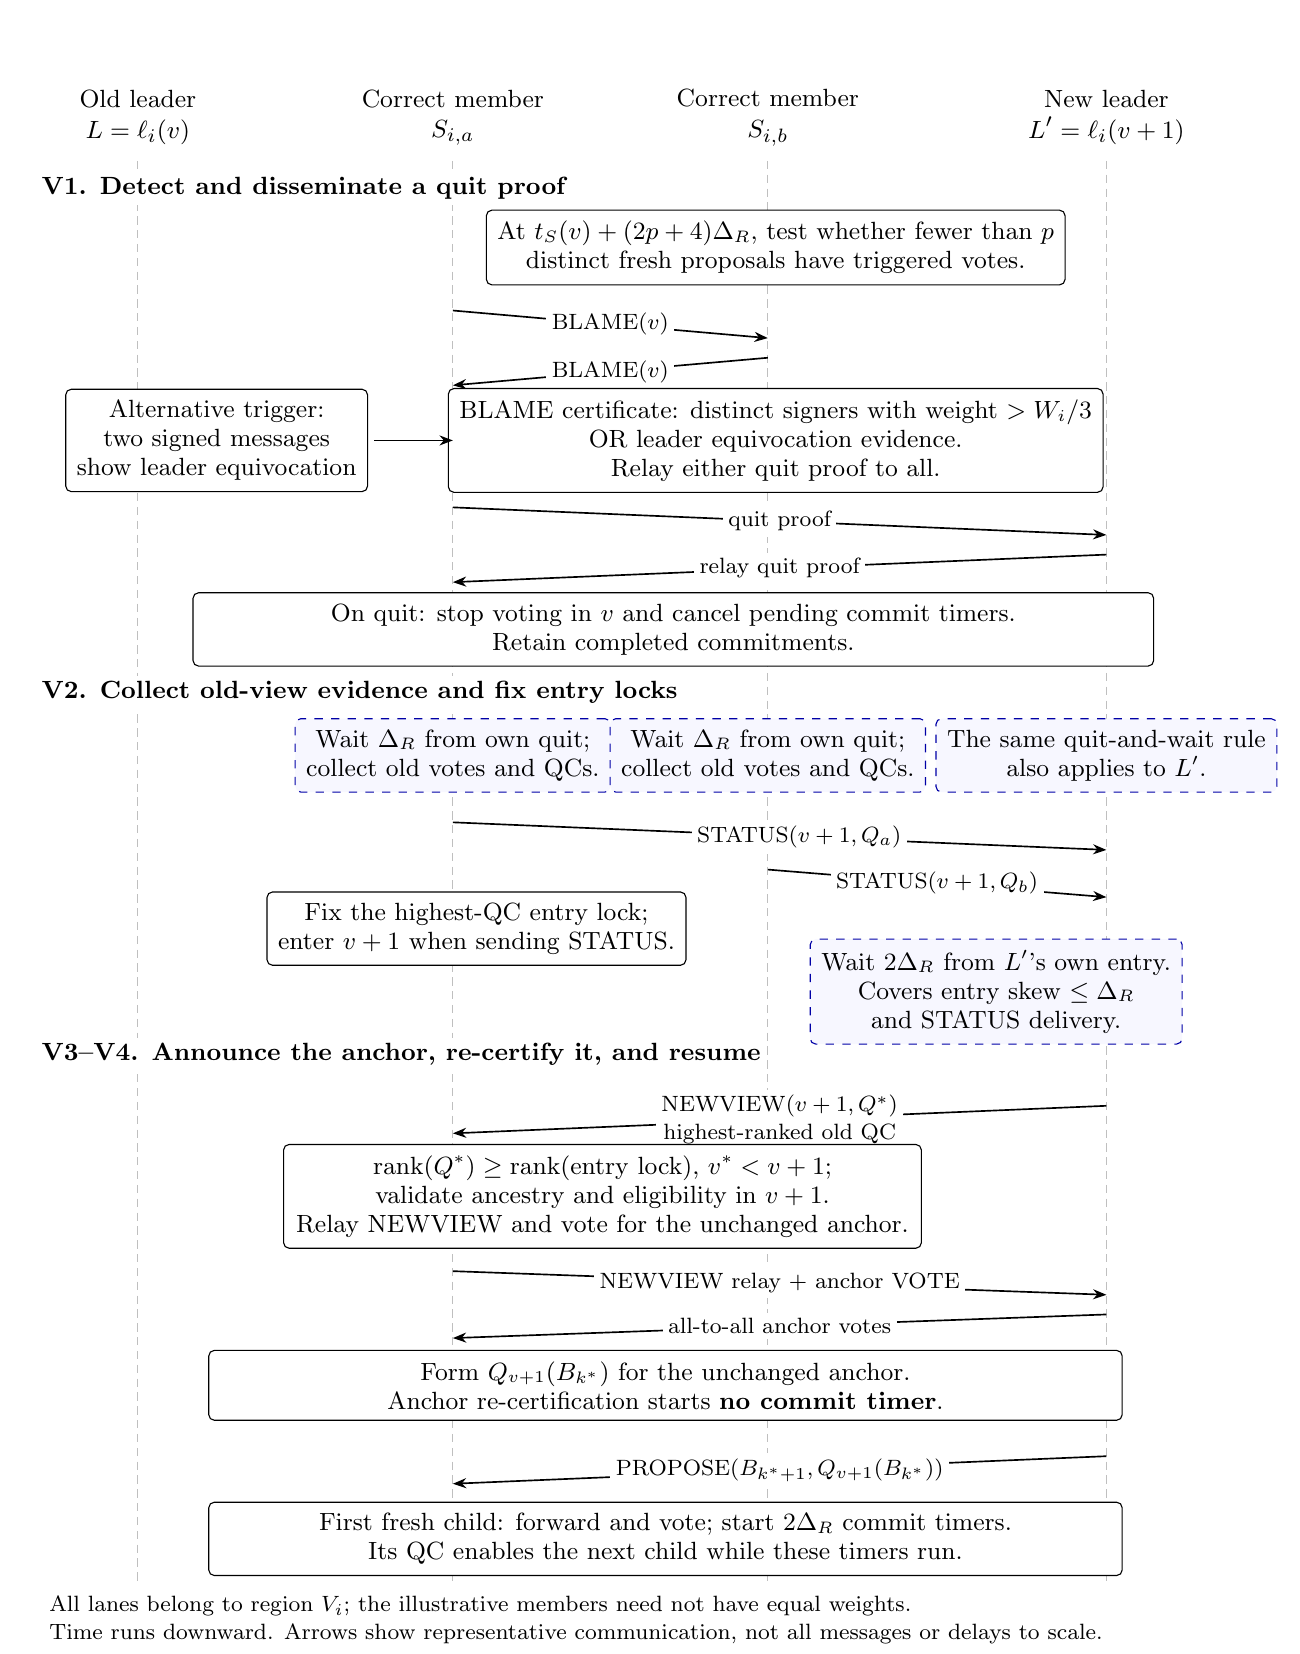
\begin{tikzpicture}[
  x=1cm,y=-1cm,font=\fontsize{9.5}{11}\selectfont,
  msg/.style={-{Stealth[length=1.7mm]},semithick},
  lane/.style={draw=black!25,densely dashed},
  label/.style={fill=white,inner sep=2pt,align=center,
    font=\fontsize{8.5}{10}\selectfont},
  phase/.style={anchor=west,font=\fontsize{9.5}{11}\selectfont\bfseries,
    fill=white,inner sep=2pt},
  state/.style={draw,rounded corners=2pt,fill=white,align=center,
    inner sep=4pt,font=\fontsize{9}{10.5}\selectfont},
  wait/.style={draw=blue!65!black,dashed,rounded corners=2pt,
    fill=blue!3,align=center,inner sep=4pt,
    font=\fontsize{9}{10.5}\selectfont}
]
  \path[use as bounding box] (-.4,-.65) rectangle (15.4,19.65);
  \node[align=center] at (1.0,0) {Old leader\\$L=\ell_i(v)$};
  \node[align=center] at (5.0,0) {Correct member\\$S_{i,a}$};
  \node[align=center] at (9.0,0) {Correct member\\$S_{i,b}$};
  \node[align=center] at (13.3,0) {New leader\\$L'=\ell_i(v+1)$};
  \foreach \x in {1,5,9,13.3} \draw[lane] (\x,.55)--(\x,18.65);

  \node[phase] at (-.3,.90) {V1. Detect and disseminate a quit proof};
  \node[state] at (9.1,1.65)
    {At $t_S(v)+(2p+4)\Delta_R$, test whether fewer than $p$\\
     distinct fresh proposals have triggered votes.};
  \draw[msg] (5,2.45)--node[label] {$\mathrm{BLAME}(v)$} (9,2.80);
  \draw[msg] (9,3.05)--node[label] {$\mathrm{BLAME}(v)$} (5,3.40);
  \node[state] at (2.0,4.10)
    {Alternative trigger:\\two signed messages\\show leader equivocation};
  \node[state,minimum width=7.8cm] at (9.1,4.10)
    {BLAME certificate: distinct signers with weight $>W_i/3$\\
     OR leader equivocation evidence.\\Relay either quit proof to all.};
  \draw[msg] (4.0,4.10)--(5.0,4.10);
  \draw[msg] (5,4.95)--node[label] {quit proof} (13.3,5.30);
  \draw[msg] (13.3,5.55)--node[label] {relay quit proof} (5,5.90);
  \node[state,minimum width=12.2cm] at (7.8,6.50)
    {On quit: stop voting in $v$ and cancel pending commit timers.\\
     Retain completed commitments.};

  \node[phase] at (-.3,7.30) {V2. Collect old-view evidence and fix entry locks};
  \node[wait] at (5,8.10)
    {Wait $\Delta_R$ from own quit;\\collect old votes and QCs.};
  \node[wait] at (9,8.10)
    {Wait $\Delta_R$ from own quit;\\collect old votes and QCs.};
  \node[wait] at (13.3,8.10)
    {The same quit-and-wait rule\\also applies to $L'$.};
  \draw[msg] (5,8.95)--node[label,pos=.53] {$\mathrm{STATUS}(v+1,Q_a)$} (13.3,9.30);
  \draw[msg] (9,9.55)--node[label] {$\mathrm{STATUS}(v+1,Q_b)$} (13.3,9.90);
  \node[state] at (5.3,10.30)
    {Fix the highest-QC entry lock;\\enter $v+1$ when sending STATUS.};
  \node[wait] at (11.9,11.10)
    {Wait $2\Delta_R$ from $L'$'s own entry.\\
     Covers entry skew $\leq\Delta_R$\\and STATUS delivery.};

  \node[phase] at (-.3,11.90) {V3--V4. Announce the anchor, re-certify it, and resume};
  \draw[msg] (13.3,12.55)--node[label,pos=.50]
    {$\mathrm{NEWVIEW}(v+1,Q^*)$\\highest-ranked old QC} (5,12.90);
  \node[state,minimum width=8.1cm] at (6.9,13.70)
    {$\operatorname{rank}(Q^*)\geq\operatorname{rank}(\mathrm{entry\ lock})$,
     $v^*<v+1$;\\validate ancestry and eligibility in $v+1$.\\
     Relay NEWVIEW and vote for the unchanged anchor.};
  \draw[msg] (5,14.65)--node[label] {NEWVIEW relay + anchor VOTE} (13.3,14.95);
  \draw[msg] (13.3,15.20)--node[label] {all-to-all anchor votes} (5,15.50);
  \node[state,minimum width=11.6cm] at (7.7,16.10)
    {Form $Q_{v+1}(B_{k^*})$ for the unchanged anchor.\\
     Anchor re-certification starts \textbf{no commit timer}.};
  \draw[msg] (13.3,17.00)--node[label,pos=.50]
    {$\mathrm{PROPOSE}(B_{k^*+1},Q_{v+1}(B_{k^*}))$} (5,17.35);
  \node[state,minimum width=11.6cm] at (7.7,18.05)
    {First fresh child: forward and vote; start $2\Delta_R$ commit timers.\\
     Its QC enables the next child while these timers run.};
  \node[align=left,font=\fontsize{8.5}{10}\selectfont,anchor=west] at (-.25,19.08)
    {All lanes belong to region $V_i$; the illustrative members need not have equal weights.\\
     Time runs downward. Arrows show representative communication, not all messages or delays to scale.};
\end{tikzpicture}
}
\caption{Regional blame and view-change communication. A blame quorum or
leader-equivocation proof causes view exit. Each member waits $\Delta_R$
from its own exit before sending STATUS; the new leader waits $2\Delta_R$
from its own entry before announcing NEWVIEW. Re-certifying the unchanged
anchor starts no commit timer; the first fresh child resumes the pipeline.
Time runs downward, and arrows show representative transmissions.}
\label{fig:change}
\end{figure}

The list $\mathcal L_i$ specifies who replaces a failed producer. Planned
producer rotation, if later required, must invoke this safe handover rather
than reset the log or discard a committed prefix; no separate planned-tenure
mechanism is added in this version.

\subsection{Confirmation receipts and slashing}\label{sec:receipt}
After committing $B_k$, an honest member signs a CONFIRM statement binding
the session, block digest and position, and sends it to peers and subscribed
consumers. Matching CONFIRM endorsements from distinct members of weight
$>W_i/3$, with the block and any missing ancestry, form the receipt $\pi_h$
for its committed prefix. CONFIRM signatures are domain-separated from VOTE
and follow the local commit rule. A raw vote QC is not a receipt.

Let $D=(\mathit{chainId},\mathit{contract},\mathit{cfgId},i,\mathit{sid})$
identify the chain, adjudicating contract, fixed configuration, region and
regional session. Signed statements bind $D$ through their authorization
context. Headers use a canonical encoding; a mini-block's identity remains
$q_h=\Hash(\Tag{MINIBLOCK},H_h)$, independent of signature encoding.

\begin{definition}[Leader double-head evidence]\label{def:double-head}
Write $\operatorname{ctx}(H)=(D,v,h)$ for an ORDER header's authorization
context, original producing view and mini-block height. Let
$E=(H,H',\sigma,\sigma')$, where $\sigma$ and $\sigma'$ are signatures by
the same producer key $S$. Then $E$ is valid double-head evidence if
\[
 \begin{gathered}
 \operatorname{ctx}(H)=\operatorname{ctx}(H')=(D,v,h),
 \qquad S=\ell_i(v)\text{ in the configuration identified by }D,\\
 \operatorname{Verify}_{S}(\Tag{ORDER},H,\sigma)
 =\operatorname{Verify}_{S}(\Tag{ORDER},H',\sigma')=1,\\
 \Hash(\Tag{MINIBLOCK},H)\ne\Hash(\Tag{MINIBLOCK},H').
 \end{gathered}
\]
\end{definition}
The two authenticated headers suffice: the leader has signed different
heads for the same production opportunity, whether or not either was voted
on or committed. A different parent or transaction commitment changes the
head. No quorum certificate or proof of elapsed time is required.
The comparison uses the original producing view in the headers, not the view
of a later certificate that re-certifies their batch.

\begin{protocol}{alg:slash}{Submit and adjudicate leader double-head evidence}
\textbf{Input:} evidence $E$ and the configuration referenced by $D$.
\begin{enumerate}[label=\textbf{E\arabic*.}]
\item \textbf{Submit.} Any observer may submit the two original signed
headers to the L1 adjudicator.
\item \textbf{Verify.} Require $D$ to name this chain and adjudicating
contract. Resolve its session and historical configuration from the
contract's authorized records; check canonical encoding, producer
authorization and every condition of \cref{def:double-head}. Reject evidence
failing any check.
\item \textbf{Deduplicate.} Compute the offense identifier
\[
 o=\Hash(\Tag{DOUBLEORDER},D,S,v,h).
\]
Skip an already adjudicated $o$. This slot-level identifier prevents repeated
penalties from reordered evidence, alternative signatures or additional
conflicting heads at the same slot.
\item \textbf{Apply.} Atomically record $o$ and impose the configured L1
equivocation penalty on $S$. Retain the evidence; membership and weights
remain fixed until an authorized configuration transition.
\end{enumerate}
\end{protocol}

The remaining signed comparison domains protect the corresponding rules:
\begin{itemize}
\item \emph{Votes:} one member signs different block digests at the same
$D$, view and batch position.
\item \emph{Leader proposals:} one leader signs incompatible
PROPOSE/NEWVIEW blocks in the same $D$ and view, or announces two different
NEWVIEW anchors for that view. Two different anchors violate the single-anchor
rule even when one extends the other.
\item \emph{Confirmations:} one member endorses incompatible committed
prefixes in the same $D$, even if the endorsements originate in different
views. The evidence includes the signed endpoints and authenticated ancestry
needed to exhibit a conflicting position.
\end{itemize}
Evidence concerns the original signer; forwarding it or re-encoding a
signature does not create equivocation. Lawful cross-view re-proposals and
unchanged-anchor re-certification do not satisfy the same-view ORDER or VOTE
rules; incompatible confirmed prefixes remain evidence across views.
Silence and BLAME alone do not prove equivocation. L1 staking rules set
penalties, evidence retention and withdrawal conditions.
The unfinished CFT protocol introduces
no REPORT or FFG signing rules in this version.

\section{Stream Delivery and Data Retrieval}\label{sec:delivery}
Delivery uses the same interface whether the underlying regional engine is
Sync HotStuff or another SMR. The leader streams mini-block bodies as they
become available and pushes confirmation receipts when ready. Early bodies
can reduce transfer latency, but do not authorize \Tag{Deliver}.
Non-leader replicas retain confirmed data and expose their confirmed frontier.

\begin{protocol}{alg:retrieval}{Leader stream with peer poll-fetch}
\begin{enumerate}[label=\textbf{D\arabic*.}]
\item \textbf{Push.} Receive the leader's stream of bodies and receipts.
Verify content commitments and buffer objects whose confirmation or predecessor
is missing. Append only a verified contiguous confirmed prefix.
\item \textbf{Poll.} A gap, missing receipt, or periodic poll asks regional
peers for their confirmed frontier. Treat an unsigned tip or bare digest as
a retrieval hint; advancement requires a verifiable receipt.
\item \textbf{Fetch.} Request the missing range and proof from a holder,
trying other configured members after a timeout. Requests and replies have
bounded size; split larger gaps into consecutive ranges.
\item \textbf{Verify and resume.} Check \Proc{VerifyStream}, original producer
authorization, commitments and predecessor continuity. Cache verified objects
and emit each previously undelivered position once. A faulty relay can delay
delivery but cannot change accepted contents.
\end{enumerate}
\end{protocol}

\begin{figure}[H]\centering
% Data availability and transport are separate from the consensus decision.
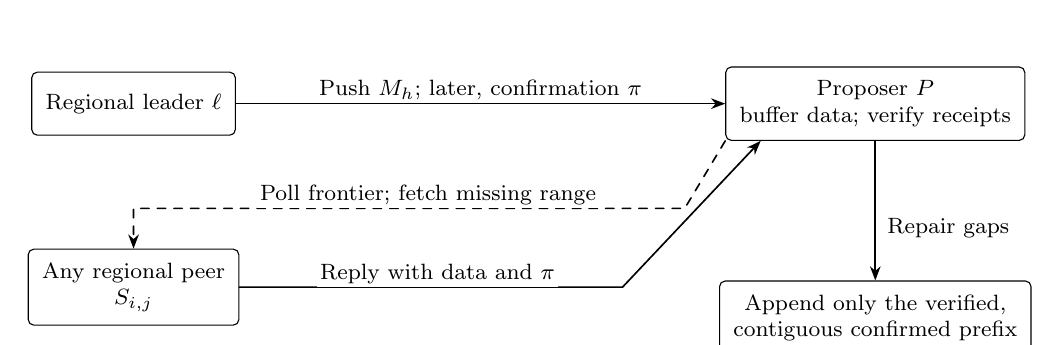
\begin{tikzpicture}[
  x=1cm,y=1cm,font=\footnotesize,line cap=round,line join=round,
  flow/.style={-{Stealth[length=1.8mm]},semithick},
  request/.style={flow,dashed},
  box/.style={draw,rounded corners=2pt,align=center,fill=white,inner sep=5pt},
  lab/.style={fill=white,inner sep=1pt,align=center}
]
  \node[box,minimum width=2.13cm,minimum height=.80cm] (leader) at (1.43,2.80)
    {Regional leader $\ell$};
  \node[box,minimum width=3.78cm,minimum height=.80cm] (proposer) at (10.85,2.80)
    {Proposer $P$\\buffer data; verify receipts};
  \draw[flow] (leader.east) -- node[lab,above] {Push $M_h$; later, confirmation $\pi$} (proposer.west);

  \node[box,minimum width=2.13cm,minimum height=.91cm] (peer) at (1.43,.47)
    {Any regional peer\\$S_{i,j}$};
  \draw[request] (proposer.south west) -- (8.43,1.47) -- (1.43,1.47) -- (peer.north);
  \node[lab,above] at (5.17,1.47) {Poll frontier; fetch missing range};
  \draw[flow] (peer.east) -- (7.64,.47) -- ($(proposer.south west)+(.45,0)$);
  \node[lab,above] at (5.29,.47) {Reply with data and $\pi$};

  \node[box,minimum width=3.78cm,minimum height=.72cm] (deliver) at (10.85,.08)
    {Append only the verified,\\contiguous confirmed prefix};
  \draw[flow] (proposer.south) -- (deliver.north);
  \node[lab,anchor=west] at (10.96,1.22) {Repair gaps};
\end{tikzpicture}

\caption{Push is the primary path; polling and fetching from peers repair
missing data or receipts. All paths pass the same acceptance rule.}
\label{fig:retrieval}
\end{figure}

For the analyzed session, correct replicas retain confirmed bodies and
endorsements and answer bounded requests. A live $P$ eventually reaches such
holders; if no single node has assembled a receipt, $P$ can collect matching
endorsements from them. The model must budget this serving traffic along with
consensus. Recovery from loss of every regional copy, pruning and archive
policy require additional mechanisms. A data-fetch timeout never elects a
leader or grants a different region production authority.

\section{Security of the Regional SMR}\label{sec:security}
The following arguments concern one activated stake configuration under
\cref{ass:network}. They specialize the temporal safety argument of
Sync HotStuff~\cite{synchotstuff} to weights and the mini-block application.
Correct nodes preserve votes, committed prefixes and view state across any
permitted restart.

\begin{lemma}[Certificate and handover preservation]\label[lemma]{lem:preserve}
If a correct member directly commits $B_k$ in view $v$, no conflicting block
is certified in that view, and every correct member enters view $v+1$ with
an entry lock of rank at least $(v,k)$.
\end{lemma}
\begin{proof}
Suppose the timer expires at time $t$. Its owner forwarded and voted for
$B_k$ at $t-2\Delta_R$, so all correct members receive the proposal by
$t-\Delta_R$. An earlier honest vote for a conflicting proposal would carry
leader-signed conflict evidence back to the timer owner by $t$, forcing it
to quit. A correct member that had already quit by $t-\Delta_R$ would
likewise propagate its quit proof by $t$. Both contradict this commitment.
View-entry skew is at most $\Delta_R$: the first correct quitter relays its
proof, all others quit within one delay, and each then waits one delay.

Thus all correct members can vote for this proposal by $t-\Delta_R$,
without a conflicting vote in that view. Their weight exceeds $2W_i/3$, so
each obtains $Q_v(B_k)$ by $t$. Every vote certificate contains an honest signer;
therefore no conflicting block can certify. The wait before STATUS ensures
a member entering the next view has this certificate or one of higher rank.
\end{proof}

\begin{lemma}[Unique extension across views]\label[lemma]{lem:extension}
After a correct direct commitment of $B$, every certificate of equal or
higher rank identifies $B$ or a descendant.
\end{lemma}
\begin{proof}
The same-view case follows from \cref{lem:preserve} and parent certification.
Suppose the lowest-ranked counterexample in a later view exists. Its quorum
contains an honest voter. If that vote re-certifies a NEWVIEW anchor, the
older certificate selected by NEWVIEW has rank at least the voter's lock,
hence at least the commitment rank, but below the alleged first counterexample.
It would already be a counterexample. If the vote is for a fresh proposal,
its same-view certified parent is a lower-ranked counterexample. Both cases
are impossible. Monotone entry locks preserve the induction.
\end{proof}

\begin{theorem}[SMR and stream safety]\label[theorem]{thm:safety}
Correct replicas have compatible committed block logs. Their command
projections satisfy SMR safety, and correct consumers satisfy the authenticity
and prefix-safety clauses of \cref{def:stream}.
\end{theorem}
\begin{proof}
A direct commitment preserves every earlier direct commitment by
\cref{lem:extension}; committing ancestors preserves the same order.
Hence no position has two committed blocks. Projection fixes both the
batch-command sequence and mini-block sequence. Receipt weight $>W_i/3$
exceeds faulty weight, so each receipt contains an honest post-commit
endorsement. Signature verification and hash
binding fix producer authority, transaction order and ancestry, while the
consumer appends only contiguous entries. Retrieval changes the supplier,
not the verified value.
\end{proof}

\begin{theorem}[Progress and delivery]\label[theorem]{thm:progress}
With sufficient service capacity, all correct members keep committing blocks.
Every such committed prefix is eventually delivered to live consumers.
Under the input-service clause of \cref{ass:service}, the command log also
satisfies request-level SMR liveness.
\end{theorem}
\begin{proof}
After a quit, entry times differ by at most $\Delta_R$. An honest new leader
waits $2\Delta_R$, so it learns every correct entry lock and selects an anchor
that passes all their rank checks. Re-certification produces its current-view
certificate, after which the leader can propose every $2\Delta_R$ or faster.
Even for the earliest entrant, the first fresh proposal triggers a vote by
$6\Delta_R$ after entry, and the $p$th by $(2p+4)\Delta_R$. Timely arrivals
precede deadline tests, so honest members never blame this leader; faulty
weight alone cannot reach the $>W_i/3$ threshold. Thus no BLAME certificate
can force it to quit, and its proposals commit after their timers.

A Byzantine leader either sustains this proposal progress or causes a quit
through a missed deadline or equivocation. If view changes continue, the
cyclic list reaches an honest leader; if they stop, the continuing
nonconflicting proposal chain commits. A prefix committed at only some
members survives handover and is committed everywhere through a later
descendant. Honest members alone can supply the $>W_i/3$ weight required
for BLAME and, after commitment, matching confirmations. Dissemination and
poll-fetch ensure delivery. Finally, a persistently
submitted eligible command selected in an honest-serving interval is included
in a committed batch. This last step uses the stated input-service condition,
not an inferred anti-censorship guarantee.
\end{proof}

Positive conflict evidence attributes incompatible signed statements to a
registered key. This establishes the soundness of the specified evidence
predicates, not a claim that every service failure is slashable. The proof
does not establish an outer CFT algorithm or safety after the regional
synchrony/stake assumptions fail.

\section{Complexity Analysis}\label{sec:complexity}
Let $n=|V_i|$, let $b$ bound one batch's new body bits, and let $\kappa$ bound
a signature and signer identifier. A vote, a vote certificate and a
post-commit receipt are accounted for separately.

\begin{table}[H]\centering\small
\begin{tabularx}{\textwidth}{@{}p{.32\textwidth}Y@{}}\toprule
Quantity & Bound and measurement point\\\midrule
Regional good-case commitment &
$\delta_R+2\Delta_R$ from a ready proposal, in steady state.\\
Confirmation at $P$ &
$\delta_R+2\Delta_R+\delta_P$ with its body/ancestry already available or
transferred within the same complete-object bound.\\
Pipeline interval &
Approximately $2\delta_R$ for a ready next batch; timer waits overlap.
Batch construction and offered load can increase this interval.\\
Handover to an honest successor &
$O(\Delta_R)$ after a quit proof, plus the new proposal's commitment.
Detection, additional failed successors and state acquisition are separate.\\
One bounded repair &
At most $(a+1)\theta$ after the first request, if $a$ suppliers fail before
an honest holder responds within the complete request/reply deadline $\theta$.
Polling adds at most its period plus the relevant path delay.\\\bottomrule
\end{tabularx}
\caption{Internal commitment, proof delivery, proposal spacing and repair
measure different paths. There is no cross-region finality bound yet.}
\end{table}

\textbf{Steady-state communication.}
Proposal forwarding and votes use $O(n^2)$ point-to-point transmissions per
batch. With unaggregated parent certificates, their conservative control cost
is $O(n^3\kappa)$ bits; blindly forwarding the full body adds $O(n^2b)$.
Caching and compact certificates can reduce bytes, but their setup, signer
information and retrieval cost must then be counted. Confirmation endorsements
add $O(n^2\kappa)$ regional bits and $O(n\kappa)$ per subscribed $P$.
No linear-communication claim is made for this all-to-all instantiation.

\textbf{Recovery and retrieval.}
BLAME-certificate propagation, STATUS and NEWVIEW cost at most
$O(n^2)$ transmissions and $O(n^3\kappa)$ control bits per replacement with
signature lists, in addition to the missing block data. Re-certification adds
one vote exchange. Polling and fetching depend on receiver count, missing
bytes and failed attempts; they are not free per-batch traffic.
Retention grows with the confirmed history. All bounds exclude Byzantine
wire flooding outside the admitted workload and presume enough bandwidth
and processing to satisfy the chosen delay bounds.

\begin{thebibliography}{9}\small
\setlength{\itemsep}{3pt}
\bibitem{synchotstuff}
I. Abraham, D. Malkhi, K. Nayak, L. Ren, and M. Yin.
\emph{Sync HotStuff: Simple and Practical Synchronous State Machine Replication}.
IEEE Symposium on Security and Privacy, 2020.
This draft uses the 4 May 2020 ePrint revision, Section II, Figures 1--2.
\url{https://eprint.iacr.org/2019/270}.
\bibitem{schneider}
F. B. Schneider.
\emph{Implementing Fault-Tolerant Services Using the State Machine Approach:
A Tutorial}. ACM Computing Surveys 22(4), 299--319, 1990.
\url{https://www.cs.cornell.edu/fbs/publications/SMSurvey.pdf}.
\bibitem{poscompiler}
J. Komatovic, A. Lewis-Pye, J. Neu, T. Roughgarden, and E. N. Tas.
\emph{From Permissioned to Proof-of-Stake Consensus}.
AFT 2025, LIPIcs 354, 18:1--18:26.
\url{https://doi.org/10.4230/LIPIcs.AFT.2025.18}.
\end{thebibliography}
\end{document}
